\documentclass[11pt]{report}
\usepackage[italian]{babel}
\usepackage[utf8]{inputenc}
\usepackage{graphicx}
\graphicspath{ {images/} }
\usepackage{caption}
\usepackage{subcaption}
\usepackage{float}
\usepackage{tabularx}
\usepackage[width=150mm,top=35mm,bottom=25mm,bindingoffset=6mm]{geometry}
\usepackage{fancyhdr}
\usepackage{wrapfig}
\usepackage{listings}
\usepackage{color}
\pagestyle{fancyplain}% <- use fancyplain instead fancy
\fancyhf{}
\fancyhead[R]{\thepage}
\renewcommand{\headrulewidth}{0pt}
\setlength{\headheight}{14pt}

\usepackage{xparse}

\definecolor{dkgreen}{rgb}{0,0.6,0}
\definecolor{gray}{rgb}{0.5,0.5,0.5}
\definecolor{mauve}{rgb}{0.58,0,0.82}

\lstset{frame=tb,
  language=VHDL,
  aboveskip=3mm,
  belowskip=3mm,
  showstringspaces=false,
  columns=flexible,
  basicstyle={\small\ttfamily},
  numbers=none,
  numberstyle=\tiny\color{gray},
  keywordstyle=\color{blue},
  commentstyle=\color{dkgreen},
  stringstyle=\color{mauve},
  breaklines=true,
  breakatwhitespace=true,
  tabsize=3
}

\NewDocumentCommand{\codeword}{v}{%
\texttt{#1}%
}

\usepackage[style=authoryear,sorting=none]{biblatex}
\addbibresource{references.bib}

\title{Reti Logiche}
\author{Prova Finale}
\date{Anno Accademico 2021/22}

\begin{document}
\pagenumbering{roman} 

\begin{titlepage}
    \begin{center}
        \vspace*{1cm}
        
        \Huge
        \textbf{Prova Finale - Reti Logiche}
        
        \vspace{0.5cm}
        \LARGE
    
        \textbf{Alessandro Cogollo - 10571078\\Mario Cela - 10685242}
        
        \vfill
        
        \vspace{1.8cm}
        
\includegraphics[width=50mm,scale=0.5]{images/logo.png}
        \vspace{1.0cm}
        \large
        \\Consegna 01 Dicembre 2022
        
    \end{center}
    
\end{titlepage}

\tableofcontents

\chapter{Introduzione}
\pagenumbering{arabic} 
Il gruppo di lavoro è composto dagli studenti: Alessandro Cogollo (Cod. Persona: 10571078, Matricola: 938296) e Mario Cela (Cod. Persona: 10685242, Matricola: 937675).

\section{Descrizione globale del progetto}

Il progetto consiste nella realizzazione in linguaggio VHDL di una componente hardware in grado di dialogare con una memoria RAM (descritta nel dettaglio nella sezione successiva), ed elaborare un flusso di bit generato dalla lettura delle parole salvate nella suddetta memoria. Il flusso di bit in output dal convolutore dovrà poi essere salvato in memoria a partire da un dato indirizzo.\\\\
In altre parole, l’hardware da progettare può essere modellizzato con due componenti tra loro strettamente interconnesse: un convolutore di Viterbi, e la struttura di supporto deputata al dialogo con la RAM, alla generazione del bitstream a partire dalle parole di memoria, e al salvataggio delle parole in output.


\section{Note sulla specifica}
Alcune note sulla specifica, fondamentali per la comprensione progettazione dell’hardware, sono riportate in questa sezione.
\\\\
Il modulo inizierà l’elaborazione quando il segnale \codeword{i_start} viene portato a 1, mentre consideriamo terminata l’esecuzione quando \codeword{o_done} viene portato a 1. Ulteriori note sulla relazione tra \codeword{i_start} e \codeword{o_done} sono illustrate nell’apposita sezione relativa all’interfaccia del componente.
\\\\
L’hardware deve quindi essere progettato per poter codificare più flussi in serie; ad ogni nuova elaborazione, il convolutore viene portato nel suo stato iniziale (\textbf{S\_IDLE}), così come vengono reinizializzati gli indirizzi di lettura e scrittura.
\\\\
Assumiamo infine che prima della prima codifica verrà sempre ricevuto dal componente un segnale di \codeword{i_rst}, mentre una seconda elaborazione non dovrà attendere il reset del modulo, ma solo il termine dell’elaborazione.
\\\\
Assumiamo infine che la dimensione massima della sequenza di ingresso sia di 255 byte.


\section{Struttura del convolutore}
Il convolutore rappresenta il cuore del progetto, e il suo funzionamento schematico è riportato in figura qui sotto; il rapporto di codifica utilizzato è 1/2.
\begin{center}
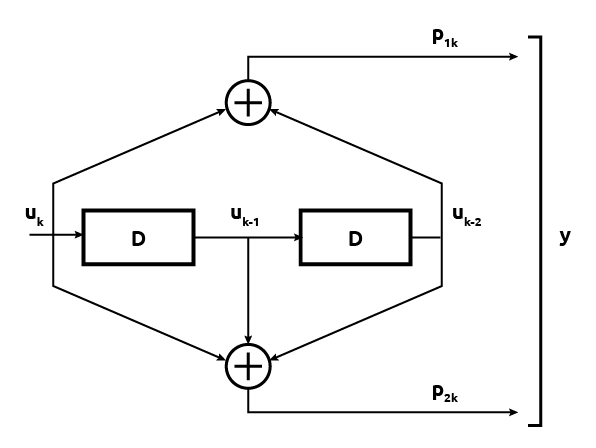
\includegraphics[width=0.7\textwidth]{images/Convolutore.png}
\end{center}

In ingresso al convolutore viene fornito un bitstream che chiameremo \textit{U}, mentre in uscita vengono generati due bitstream \textit{$P_1$} e \textit{$P_2$}. Nello specifico del problema in questione, l’uscita \textit{Y} è composta dall’alternanza, nell’ordine, di \textit{$P_1$} e \textit{$P_2$} (mostrati in figura). Il convolutore è composto da due flip-flop di tipo D; la codifica convoluzionale descritta è considerabile come un caso di codifica con memoria, in quanto l’influenza di un bit in ingresso al tempo \textit{t} si protrae sull’elaborazione di bit in input al tempo \textit{t+1} e \textit{t+2}.
\\\\
La funzione di convoluzione invece è descrivibile come segue:
\begin{center}
    $p_{1k}=u_k+u_{k-2}$
    \\
    $p_{2k}=u_k+u_{k-1}+u_{k-2}$
\end{center}
Lo schema della Finite State Machine (FSM) è riportato nella figura sottostante:

\begin{center}
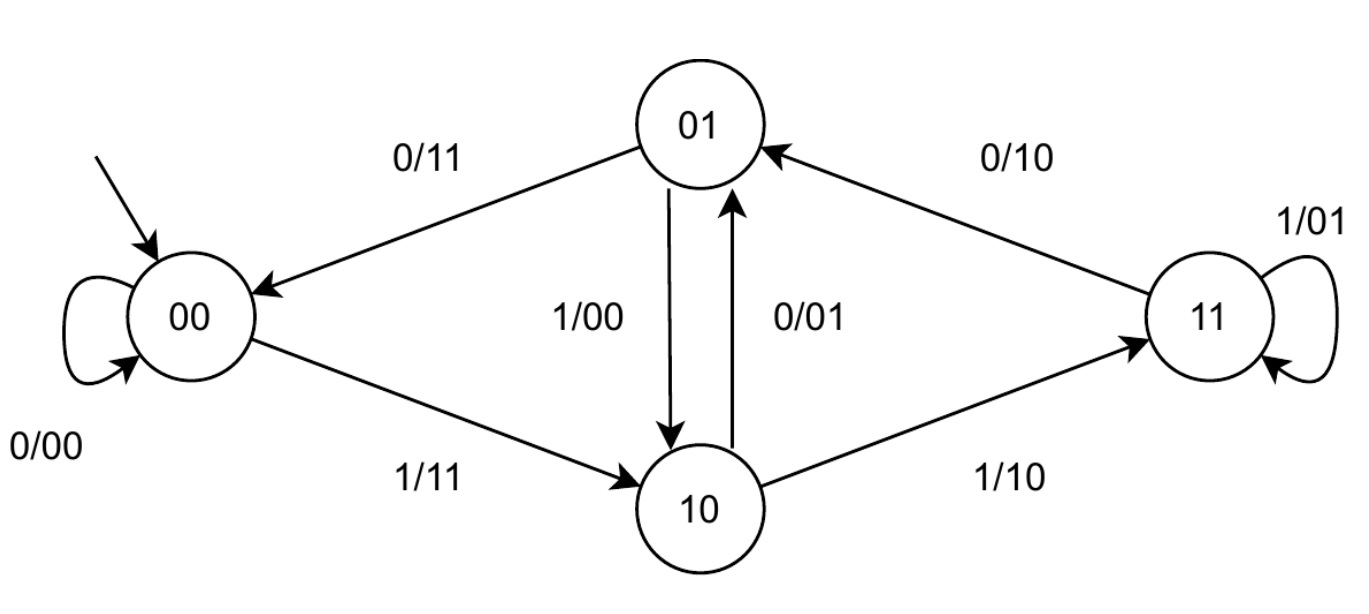
\includegraphics[width=0.89\textwidth]{images/FSM Conv.jpg}
\end{center}

Il codice convoluzionale 1/2 genera 2 bit di output a partire da un singolo bit in input, pertanto è evidente che per ogni parola letta ne verranno salvate due in memoria.


\section{Struttura della RAM}

L’hardware sintetizzato deve interfacciarsi con una memoria RAM di tipo “\textbf{Single-Port Block RAM Write-First Mode}”, in particolare la Random Access Memory è fornita dai template di Xilinx, produttore del software di simulazione e sintesi. Si tratta di una memoria RAM ad accesso \textbf{sequenziale} (single port), che \textbf{prioritizza la scrittura rispetto alla lettura} (write-first mode); entrambe le proprietà vengono specificate in quanto costituiscono casistiche limite che hanno influito sulla progettazione della componente, e nella scrittura dei casi di test, come spiegato nella sezione dedicata.
\\\\
L’interfaccia della memoria è riportata di seguito:\\
\begin{lstlisting}
port(
    clk : in std_logic;
	 we : in std_logic;
	 en : in std_logic;
	 addr : in std_logic_vector(15 downto 0);
	 di : in std_logic_vector(7 downto 0);
	 do : out std_logic_vector(7 downto 0)
);
\end{lstlisting}

L’indirizzamento della parola avviene grazie al segnale \codeword{addr}, che è rappresentato da un array di 16 bit, mentre \codeword{we} ed \codeword{en} costituiscono i segnali di accesso alla memoria, rispettivamente in scrittura ed in lettura; l’accensione del segnale di scrittura richiede l’accensione del segnale di lettura. \codeword{clk} propaga il segnale di clock, mentre \codeword{di} e \codeword{do} rappresentano i segnali in input e output alla memoria.
Da specifica, la memoria può essere idealmente divisa in due parti:

\begin{itemize}
    \item \textbf{Input}: all’indirizzo 0: si trova il numero di parole di input attese, mentre agli indirizzi successivi (fino all’indirizzo 1000 escluso) si trovano le parole che dovranno essere effettivamente elaborate.
    \item \textbf{Output}: dall’indirizzo 1000 alla fine della memoria si riserva lo spazio per la scrittura delle parole elaborate.
\end{itemize}
Un esempio di caricamento della RAM è riportato nella tabella a seguire:
\begin{center}
\begin{tabularx}{\textwidth} {
    | >{\raggedright\arraybackslash}X
    | >{\centering\arraybackslash}X
    | >{\raggedleft\arraybackslash}X | }
    \hline
    Indirizzo           & Parola (binary) & Valore (decimal) \\
    \hline\hline
    0000 0000 0000 0000 & 0000 0011       & 3                \\
    \hline
    0000 0000 0000 0001 & 0111 0000       & 112              \\
    \hline
    0000 0000 0000 0010 & 1010 0100       & 164              \\
    \hline
    0000 0000 0000 0011 & 0010 1101       & 45               \\
    \hline
    [\dots]             & [\dots]         & [\dots]          \\
    \hline
    0000 0011 1110 1000 & 0011 1001       & 57               \\
    \hline
    0000 0011 1110 1001 & 1011 0000       & 176              \\
    \hline
    0000 0011 1110 1010 & 1101 0001       & 209              \\
    \hline
    0000 0011 1110 1011 & 1111 0111       & 247              \\
    \hline
    0000 0011 1110 1100 & 0000 1101       & 13               \\
    \hline
    0000 0011 1110 1101 & 0010 1000       & 40               \\
    \hline
    \hline
\end{tabularx}
\end{center}

\section{Interfaccia del componente}
La specifica del componente richiede che l’interfaccia dell’hardware da implementare sia dotata dei seguenti segnali in ingresso (\codeword{i_}) e uscita (\codeword{o_}).
\\
\begin{lstlisting}
port (
	i_clk : in std_logic;
	i_rst : in std_logic;
	i_start : in std_logic;
	i_data : in std_logic_vector(7 downto 0);
	o_address : out std_logic_vector(15 downto 0);
	o_done : out std_logic;
	o_en : out std_logic;
	o_we : out std_logic;
	o_data : out std_logic_vector (7 downto 0)
);
\end{lstlisting}

In particolare, \codeword{i_clk} è il segnale di clock in ingresso (generato dal TestBench); garantisce un fronte di salita comune tra memoria e componente, fondamentale per eseguire correttamente i test. \codeword{i_rst} è il segnale di reset che inizializza la macchina e la prepara alla ricezione del primo segnale di start. \codeword{i_start} è il segnale di start generato dal TestBench; è richiesto dalla specifica che \codeword{i_start} rimanga alto finché \codeword{o_done} non verrà portato alto, ossia il segnale che notifica la fine dell’elaborazione. Anche il segnale di done deve rimanere alto finché il segnale di start non è riportato a zero. \codeword{i_data} e \codeword{o_data} contengono le parole di memoria in input e output verso la RAM, mentre \codeword{o_address}, \codeword{o_en}, e \codeword{o_we} sono state descritte in precedenza.


\section{Esempio di funzionamento}
Un esempio del funzionamento atteso dal componente è il seguente:

\begin{center}

    \begin{tabularx}{\textwidth}{
        | >{\raggedright\arraybackslash}X
        | >{\raggedright\arraybackslash}X
        | >{\raggedright\arraybackslash}X
        | >{\raggedright\arraybackslash}X | }
        \hline
        Indirizzo           & Parola (binary) & Valore (decimal) & Note                                    \\
        \hline\hline
        0000000000000000 & 0000 0011       & 3                & Sequenza in input       \\
        \hline
        0000000000000001 & 0111 0000       & 112              & $1^{a}$ parola di input  \\
        \hline
        0000000000000010 & 1010 0100       & 164              & $2^{a}$ parola di input \\
        \hline
        0000000000000011 & 0110 1101       & 45               & $3^{a}$ parola di input  \\
        \hline
        \dots             & \dots         & \dots          &                                         \\
        \hline
        \hline
    \end{tabularx}
\end{center}
Le parole in input \textit{W} sono tre: 01110000 10100100 00101101. Seguendo la codifica convoluzionale illustrata precedentemente, ci aspettiamo in output \textit{Z} le seguenti sei parole: 00111001 10110000 11010001 11110111 00001101 00101000, salvate in memoria come segue:
\begin{center}
    \begin{tabularx}{\textwidth}{
        | >{\raggedright\arraybackslash}X
        | >{\raggedright\arraybackslash}X
        | >{\raggedright\arraybackslash}X
        | >{\raggedright\arraybackslash}X | }
        \hline
        Indirizzo           & Parola (binary) & Valore (decimal) & Note                                 \\
        \hline\hline
        \dots              & \dots         & \dots          &                                      \\
        \hline
        0000001111101000 & 0011 1001       & 57               & $1^{a}$ parola di output   \\
        \hline
        0000001111101001 & 1011 0000       & 176              & $2^{a}$ parola di output\\
        \hline
        0000001111101010 & 1101 0001       & 209              & $3^{a}$ parola di output  \\
        \hline
        0000001111101011 & 1111 0111       & 247              & $4^{a}$ parola di output \\
        \hline
        0000001111101100 & 0000 1101       & 13               & $5^{a}$ parola di output \\
        \hline
        0000001111101101 & 0010 1000       & 40               & $6^{a}$ parola di output   \\
        \hline
        \hline
    \end{tabularx}
\end{center}

\chapter{Architettura}
\section{Segnali utilizzati}
Gli stati utilizzati dalla componente, e la loro funzione, sono elencati di seguito:
\\
\begin{lstlisting}
signal state_curr, state_future, state_last: state;
signal length, word_to_process, word_to_save: std_logic_vector (7 downto 0);
signal writing_counter  : INTEGER range 0 to 16385 := 0;
signal reading_counter    : INTEGER range 0 to 16385 := 0;
signal local_counter     : INTEGER range 0 to 8 := 0;
signal write_index       : INTEGER range 0 to 16 := 0;
constant READ_BOTTOM     : std_logic_vector (15 downto 0) := "0000000000000000";
constant WRITE_BOTTOM    : std_logic_vector (15 downto 0) := "0000001111101000";
\end{lstlisting}
I segnali \codeword{state_curr}, \codeword{state_future} e \codeword{state_last}, di tipo state, sono, come appare evidente, necessari al salvataggio dello stato corrente, futuro e passato. Lo stato corrente tiene traccia dello stato in cui si trova la FSM, ed esegue le istruzioni in esso contenute; lo stato \codeword{state_last}, invece, tiene traccia dell’ultimo stato visitato, al fine di capire la provenienza del flusso del componente, ed indirizzare correttamente ad un nuovo stato. \codeword{state_future}, infine, è necessario in quanto tra la convoluzione di un bit e l’altro, la macchina passa attraverso lo stato \textbf{S\_CONV}, è pertanto necessario tenere traccia dello stato a cui la macchina dovrà essere indirizzata dopo la visita dello stato \textbf{S\_CONV}.
\\\\
I segnali length, \codeword{word_to_process} e \codeword{word_to_save}, tutti di tipo \codeword{std_logic_vector (7 downto 0)} sono necessari per tenere traccia rispettivamente del numero di parole da leggere ed elaborare, della parola letta e da sottoporre al convolutore, e della parola elaborata e da salvare nella RAM.
\\\\
I segnali \codeword{writing_counter}, \codeword{reading_counter},  \codeword{local_counter} e \codeword{write_index} sono tutti indici e contatori necessari per indicizzare, nell’ordine, gli indirizzi di memoria su cui salvare, da cui leggere, e il numero di convoluzioni da effettuare, e i bit della parola da salvare su cui scrivere. \codeword{writing_counter} e \codeword{reading_counter} vengono sommati rispettivamente alle costanti \codeword{READ_BOTTOM} e \codeword{WRITE_BOTTOM}, ossia i valori delle porzioni iniziali e finali di memoria che indicano la parte di scrittura e lettura.

\section{Descrizione della FSM}
Viene mostrato in figura uno schema della FSM progettata:
\\
\begin{figure}[ht]
    \centering
    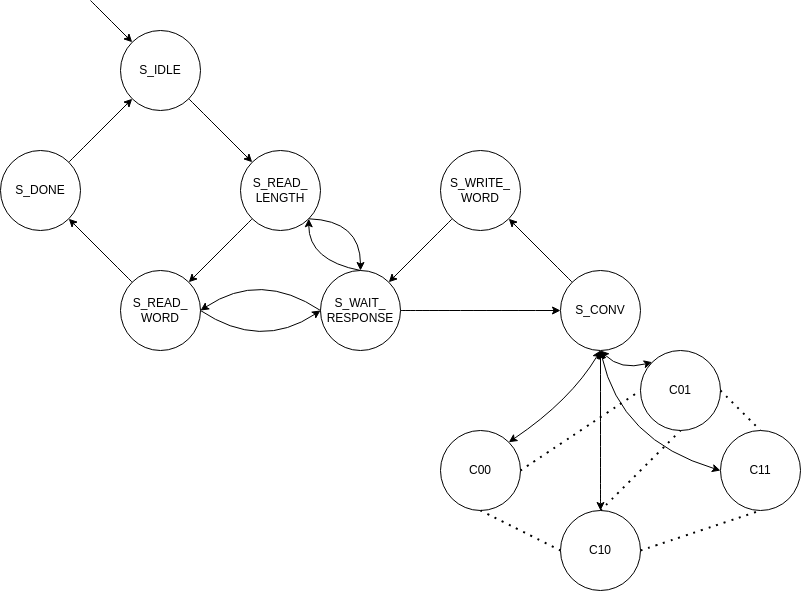
\includegraphics[width=\textwidth,height=0.74\textheight,keepaspectratio]{images/FSM.png}
    \label{fig:FSM}
\end{figure}
\\
Di seguito riportiamo gli stati utilizzati per progettare il comportamento del componente, associando ad ogni stato della FSM una specifica funzione spiegata qui sotto:
\begin{itemize}
    \item \textbf{S\_IDLE}: corrisponde allo stato di reset; vi si accede quando la componente riceve il segnale \codeword{i_rst}, serve all’inizializzazione dei valori necessari al funzionamento della macchina. Lo stato di reset persiste ad ogni giro di clock, fintanto che la componente non riceve un segnale di \codeword{i_start}.
    
    \item \textbf{S\_DONE}: corrisponde allo stato di fine elaborazione; è raggiungibile solo dallo stato \textbf{S\_READ\_WORD}, e vi si accede quando la sequenza di parole attese da elaborare è uguale al numero di parole in input elaborate. Lo stato \textbf{S\_DONE} porta alto il segnale \codeword{o_done} e abbassa invece lo stato \codeword{i_start}, raggiungendo, al successivo segnale di clock, lo stato \textbf{S\_IDLE}.
    
    \item \textbf{S\_READ\_LENGTH}: è lo stato deputato alla richiesta di lettura della lunghezza, ossia lo stato che richiede alla RAM la lettura (\codeword{o_en} = 1) della parola di memoria all’indirizzo 0000. Successivamente, reindirizza allo stato \textbf{S\_WAIT\_RESPONSE}, in attesa di risposta dalla RAM, e, al ritorno dal suddetto segnale, salva la lunghezza della sequenza attesa nello \codeword{std_logic_vector(7 downto 0)} ”length", successivamente reindirizza allo stato \textbf{S\_READ\_WORD}.
    
    \item \textbf{S\_READ\_WORD}: è lo stato deputato alla richiesta di lettura di una parola di memoria, il cui indirizzo è gestito dallo \codeword{std_logic_vector(7 downto 0)} \\ ”\codeword{reading_counter}", che viene incrementato ad ogni iterazione. Lo stato \\ \textbf{S\_READ\_WORD} si occupa inoltre di controllare se il numero di parole elaborate è minore della lunghezza di valori attesa; se così fosse, lo stato reindirizzerà allo stato \textbf{S\_WAIT\_RESPONSE}, per finalizzare la lettura (\codeword{o_en} = 1) e quindi per procedere con l'elaborazione della nuova parola; alternativamente, si verrà reindirizzati ad \textbf{S\_DONE}.
    
    \item \textbf{S\_WAIT\_RESPONSE}: è uno “stato cuscinetto”, utile in attesa della risposta della RAM, che, in quanto memoria asincrona, richiede un giro di clock per fornire alla componente interrogante una risposta di lettura e/o scrittura.
    
    \item \textbf{S\_WRITE\_WORD}: è lo stato deputato alla scrittura in memoria della parola elaborata. Vi si accede sempre e solo dallo stato \textbf{S\_CONV}, a seguito di 4 o 8 letture di bit in ingresso, ossia quando in output è pronta per il salvataggio una parola di 8 bit. Lo stato alza quindi i segnali di \codeword{o_en} e \codeword{o_we}, e provvede a scrivere all’indirizzo la cui gestione è affidata al segnale \codeword{writing_counter}, che viene incrementato ad ogni salvataggio. Successivamente si viene indirizzati allo stato \textbf{S\_WAIT\_RESPONSE}, al fine di permettere il salvataggio in memoria, e successivamente allo stato \textbf{S\_CONV} per continuare la convoluzione, o alla lettura di una nuova parola (stato \textbf{S\_READ\_WORD}), nel caso in cui siano stati consumati tutti i bit della parola in ingresso.
    
    \item \textbf{S\_CONV}: funge da controller della convoluzione, permette infatti di controllare, tra l’analisi di un bit e l’altra, se sono state eseguite 4 o 8 convoluzioni, ossia se sono state prodotte in output dal convolutore una o due parole, e se quindi è necessario andare a leggere un’ulteriore parola dalla memoria. Lo stato successivo a \textbf{S\_CONV} è, nel caso in cui siano state eseguite 4 o 8 convoluzioni, lo stato di scrittura in memoria della parola, mentre in tutti gli altri casi lo stato corrente viene indirizzato al \codeword{future_state} di cui si è tenuta traccia nell’ultima convoluzione di bit. Se il convolutore non ha mai ricevuto bit in ingresso, \codeword{future_state} sarà settato a C00.
    
    \item \textbf{C00, C01, C10, C11}: sono gli stati deputati alla convoluzione. Il loro funzionamento è descritto nel dettaglio nella sezione 1.3. Il segnale \codeword{future_state} tiene traccia del futuro stato di convoluzione da visitare, affinché vi ci si possa spostare una volta visitato lo stato \textbf{S\_CONV}, cosa che accade successivamente alla visita di ogni stato di convoluzione.
    
\end{itemize}

\chapter{Risultati Sperimentali}
\section{Sintesi}
La sintesi schematica della componente si presenta come nella figura sottostante.

\begin{center}
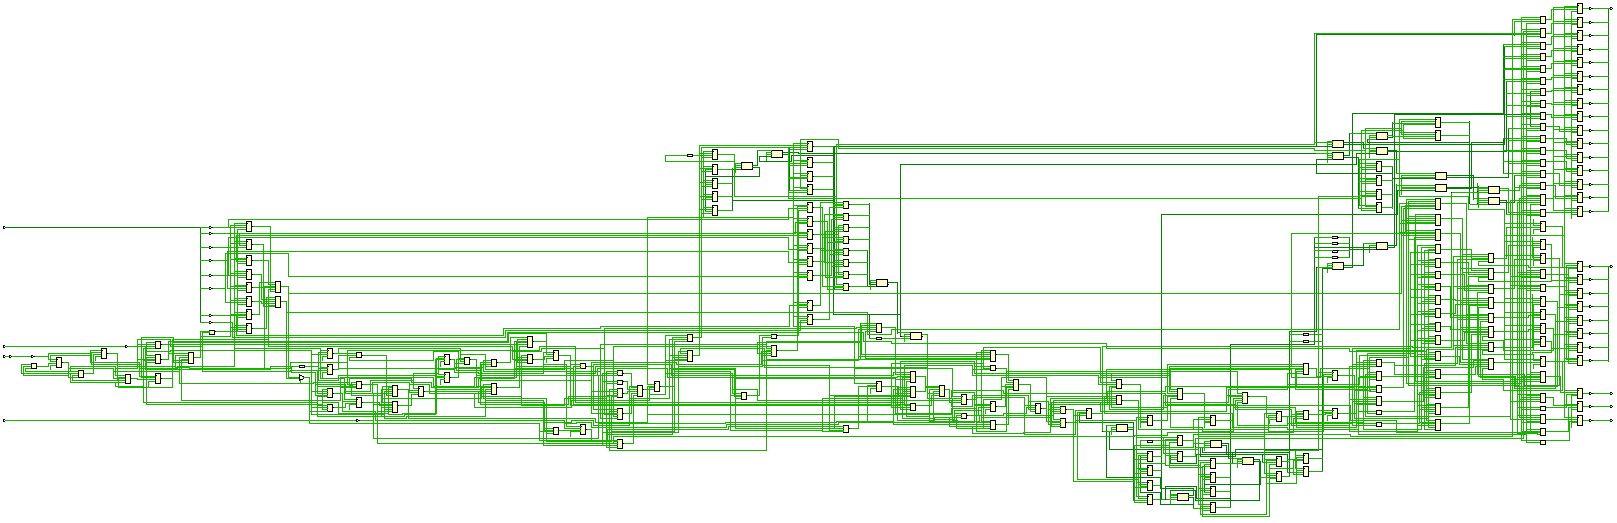
\includegraphics[width=\textwidth]{images/Schematic.png}
\end{center}

\section{Report Utilization}
Segue la tabella che descrive la slice logic della macchina a seguito della sintesi, ottenuta grazie al comando \codeword{report_utilization} fornito da Vivado:

\begin{center}
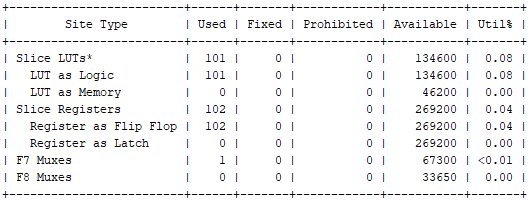
\includegraphics[width=0.8\textwidth]{images/report_uilization.png}
\end{center}

\section{Report Timing}
Da specifica, deve essere progettato un componente che sia funzionante per un tempo di clock $T_{clock}\leq 100 ns$. Il comando \codeword{report_timing_summary} mostra che il Worst Negative Slack (WNS) e il Worst Hold Slack (WHS) sono positivi, quindi il vincolo viene rispettato correttamente. Segue quanto mostrato dal report:

\begin{center}
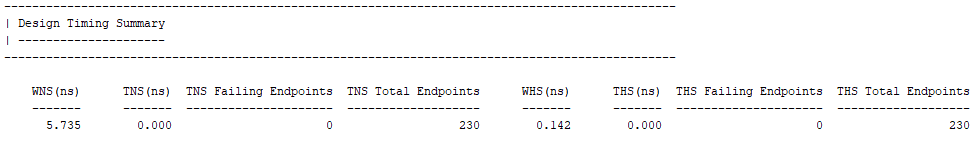
\includegraphics[width=\textwidth]{images/report_timing.png}
\end{center}

\section{Simulazioni}
Il componente progettato è stato testato per verificarne il corretto funzionamento con la sottomissione a testbench randomicamente generati, e ad ulteriori testbench contenenti i casi limite di seguito riportati: 
\begin{itemize}
    \item \textbf{Sequenza Minima}: si testa il caso in cui la parola di memoria in posizione 0000, ossia quella contenente il numero di parole di cui si richiede la lettura, sia nulla. Ci aspettiamo quindi che la convoluzione termini, e che le parole di memoria dalla cella 1000 in poi siano vuote.
    \begin{center}
    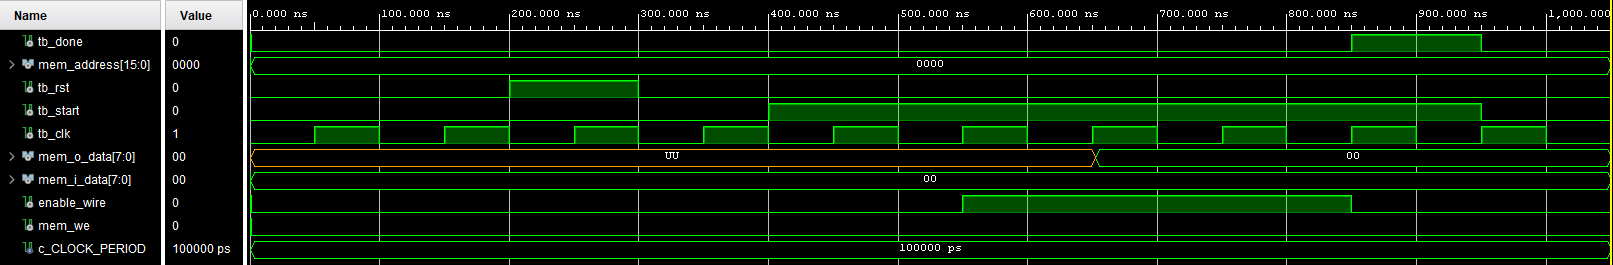
\includegraphics[width=0.93\textwidth]{images/simulations/SeqMin.png}
    \end{center}
    \item \textbf{Sequenza Massima}: si testa il caso in cui la parola di memoria in posizione 0000 contenga il numero di parole massime ricevibili in input (da specifica, 255). Al termine dell’elaborazione, agli indirizzi successivi al 1000, ci aspettiamo siano salvate le parole correttamente codificate.
    \begin{center}
    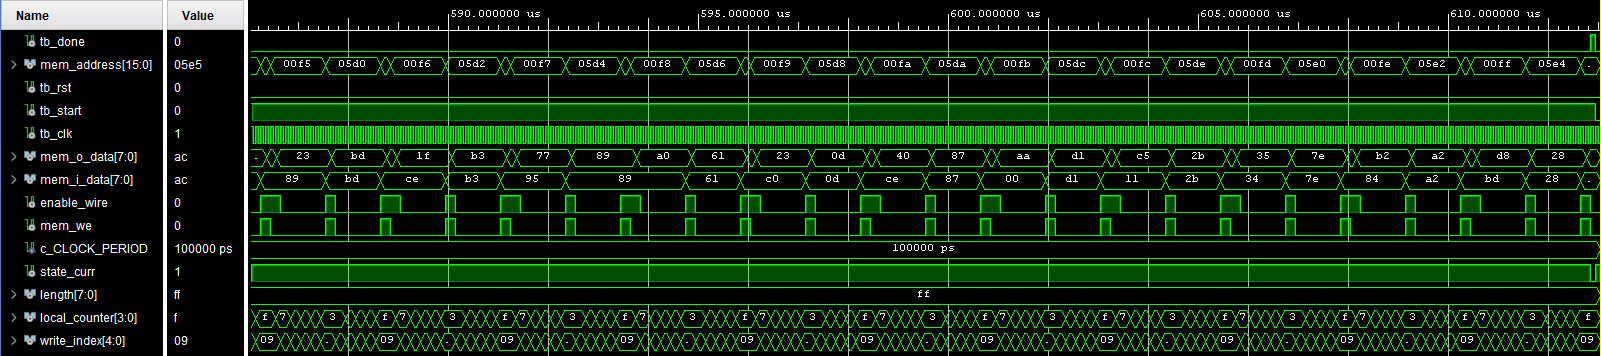
\includegraphics[width=0.93\textwidth]{images/simulations/SeqMax.png}
    \end{center}
    \item \textbf{Reset Improvviso}: il convolutore inizia la lettura della RAM, ma riceve improvvisamente un segnale di reset che riporta la componente nello stato iniziale. Ci aspettiamo che la convoluzione avvenga comunque, e che le parole salvate in memoria siano le stesse che verrebbero salvate in assenza di reset improvviso.
    \begin{center}
    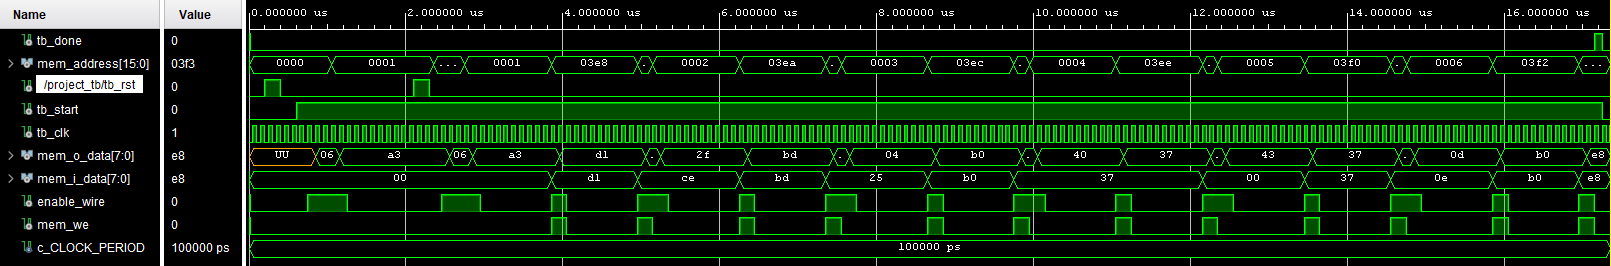
\includegraphics[width=0.93\textwidth]{images/simulations/TBReset.png}
    \end{center}
    \item \textbf{Re-Encode}:  il convolutore viene testato sottoponendolo a tre sequenze diverse di input nella stessa test bench; ci aspettiamo che la codifica avvenga correttamente per tutte e tre le sequenze.
    \begin{center}
    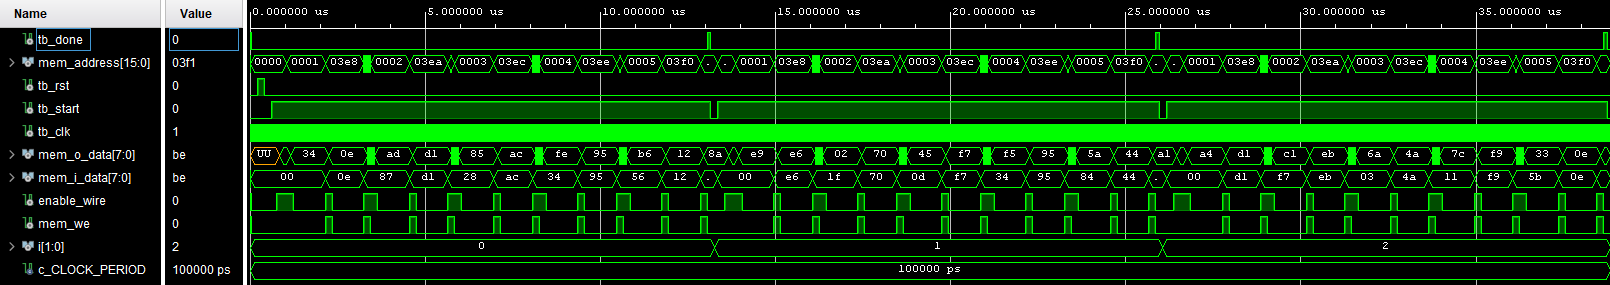
\includegraphics[width=0.93\textwidth]{images/simulations/REEncode.png}
    \end{center}
    \item \textbf{Doppio Uguale}: viene eseguito un double processing. Dopo aver inizializzato la RAM, il testbench procede col verificare che gli output sono stati corretttamente generati dalla macchina e che le parole siano state convolute correttamente. A questo punto, viene inviato un nuovo segnale di \codeword{i_start} in modo tale che la macchina elabori nuovamente le stesse parole studiate in precedenza. Viene quindi verificato che a parità di input, l’output non cambia.
    \begin{center}
    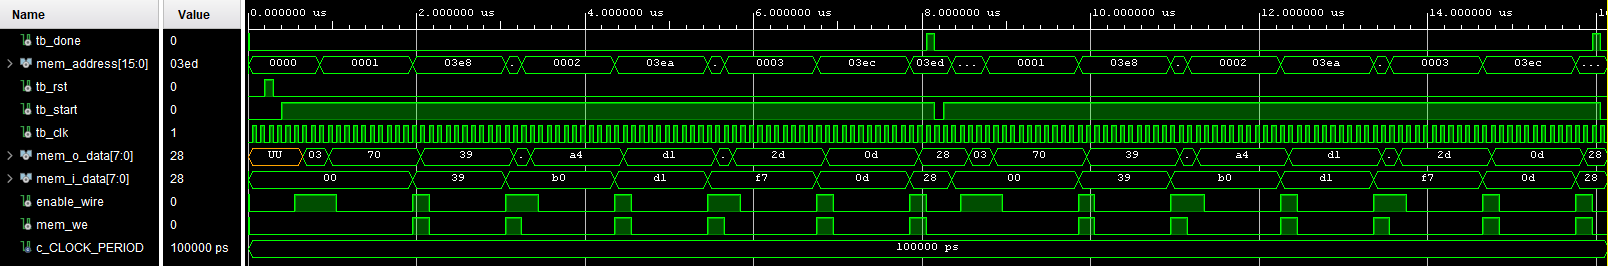
\includegraphics[width=0.93\textwidth]{images/simulations/DoppioUguale.png}
    \end{center}
\end{itemize}
Per verificare il corretto funzionamento, soprattutto in fase di progetto, sono stati utilizzati il testbench fornito dai docenti e altri test prodotti da un generatore casuale.

\chapter{Conclusioni}
Un’ottimizzazione effettuata è stata la rimozione di uno stato intermedio tra la lettura della parola di memoria e l’inizio della sua convoluzione. Abbiamo ovviato al suddetto stato indirizzando direttamente allo stato \textbf{S\_CONV}, successivo allo stato \textbf{S\_WAIT\_RESPONSE}. 

Un’eventuale ulteriore ottimizzazione potrebbe essere introdotta accorpando le funzionalità dello stato \textbf{S\_CONV} negli stati del codificatore convoluzionale (C00, C01, C10, C11), per evitare che la componente debba passare sempre attraverso uno stato “cuscinetto” tra uno stato di convoluzione e l’altro, rallentando la codifica dell’ingresso. Questa strada non è stata seguita per questioni di manutenzione del codice, infatti accorpando le funzionalità dello stato \textbf{S\_CONV} in un solo stato risulta meno dispersivo piuttosto che replicarle per tutti gli stati di convoluzione.

\section{Ulteriori note}
La versione del software utilizzato per la progettazione e sintesi è \textbf{Vivado ML 2022.2}, la FPGA target scelta, come da specifica, è stata \textbf{Artix-7 FPGA xc7a200tfbg484-1}.

\end{document}
